% XeLaTeX document
\documentclass[12pt,a4paper]{article}

% Редактируем: конфигурация, личные настройки: имя, название предмета и пр. для титульной страницы и метаданных документа здесь
\newcommand{\university}{Национальный исследовательский Университет ИТМО}
\newcommand{\mfaculty}{Мегафакультет информационных и трансляционных технологий}
\newcommand{\faculty}{Факультет инфокоммуникационных технологий}
\newcommand{\city}{Санкт-Петербург}
\newcommand{\num}{ №5}
\newcommand{\docname}{Лабораторная работа}
\newcommand{\subject}{Алгоритмы и структуры данных}
\newcommand{\tutorname}{В.Е. Артамонова}
\newcommand{\studentname}{А.И. Либерман}
\newcommand{\group}{К3124}

% Не редактируем: используемые пакеты
% настройка кодировки, шрифтов и русского языка
\usepackage{fontspec}
\usepackage{polyglossia}

% рабочие ссылки в документе
\usepackage{hyperref}

% графика
\usepackage{graphicx}
\usepackage{tikz}

% поворот страницы
\usepackage{pdflscape}

% качественные листинги кода
\usepackage{minted}
\usepackage{listings}
\usepackage{lstfiracode}

% отключение копирования номеров строк из листинга, работает не во всех просмотрщиках (в Adobe Reader работает)
\usepackage{accsupp}
\newcommand\emptyaccsupp[1]{\BeginAccSupp{ActualText={}}#1\EndAccSupp{}}
\let\theHFancyVerbLine\theFancyVerbLine
\def\theFancyVerbLine{\rmfamily\tiny\emptyaccsupp{\arabic{FancyVerbLine}}}

% библиография
\bibliographystyle{templates/gost-numeric.bbx}
\usepackage{csquotes}
\usepackage[parentracker=true,backend=biber,hyperref=true,bibencoding=utf8,style=numeric-comp,language=auto,autolang=other,citestyle=gost-numeric,defernumbers=true,bibstyle=gost-numeric,sorting=ntvy]{biblatex}

% установка полей
\usepackage{geometry}

% нумерация картинок по секциям
\usepackage{chngcntr}

% дополнительные команды для таблиц
\usepackage{booktabs}

% для заголовков
\usepackage{caption}
\usepackage{titlesec}
\usepackage[dotinlabels]{titletoc}

% разное для математики
\usepackage{amsmath, amsfonts, amssymb, amsthm, mathtools}

% водяной знак на документе, см. main.tex
\usepackage[printwatermark]{xwatermark}

% Не редактируем: параметры используемых пакетов и не только
% настройки polyglossia
\setdefaultlanguage{russian}
\setotherlanguage{english}

% локализация
\addto\captionsrussian{
	\renewcommand{\figurename}{Рисунок}%
	\renewcommand{\partname}{Глава}
	\renewcommand{\contentsname}{\centerline{Содержание}}
	\renewcommand{\listingscaption}{Листинг}
}

% основной шрифт документа
\setmainfont{CMU Serif}
\newfontfamily\cyrillicfont{CMU Serif}[Script=Cyrillic]

% перечень использованных источников
\addbibresource{refs.bib}

% настройка полей
\geometry{top=2cm}
\geometry{bottom=2cm}
\geometry{left=2cm}
\geometry{right=2cm}
\geometry{bindingoffset=0cm}

% настройка ссылок и метаданных документа
\hypersetup{unicode=true,colorlinks=true,linkcolor=red,citecolor=green,filecolor=magenta,urlcolor=cyan,
	pdftitle={\docname},
	pdfauthor={\studentname},
	pdfsubject={\subject},
	pdfcreator={\studentname},
	pdfproducer={Overleaf},
	pdfkeywords={\subject}
}

% настройка подсветки кода и окружения для листингов
\usemintedstyle{colorful}
\newenvironment{code}{\captionsetup{type=listing}}{}

% шрифт для листингов с лигатурами
\setmonofont{FiraCode-Regular.otf}[
	SizeFeatures={Size=10},
	Path = templates/,
	Contextuals=Alternate
]

% оформления подписи рисунка
\captionsetup[figure]{labelsep = period}

% подпись таблицы
\DeclareCaptionFormat{hfillstart}{\hfill#1#2#3\par}
\captionsetup[table]{format=hfillstart,labelsep=newline,justification=centering,skip=-10pt,textfont=bf}

% путь к каталогу с рисунками
\graphicspath{{fig/}}

% Внесение titlepage в учёт счётчика страниц
\makeatletter
\renewenvironment{titlepage} {
	\thispagestyle{empty}
}
\makeatother

\counterwithin{figure}{section}
\counterwithin{table}{section}

\titlelabel{\thetitle.\quad}

% для удобного конспектирования математики
\mathtoolsset{showonlyrefs=true}
\theoremstyle{plain}
\newtheorem{theorem}{Теорема}[section]
\newtheorem{proposition}[theorem]{Утверждение}
\theoremstyle{definition}
\newtheorem{corollary}{Следствие}[theorem]
\newtheorem{problem}{Задача}[section]
\theoremstyle{remark}
\newtheorem*{nonum}{Решение}

% настоящее матожидание
\newcommand{\MExpect}{\mathsf{M}}

% объявили оператор!
\DeclareMathOperator{\sgn}{\mathop{sgn}}

% перенос знаков в формулах (по Львовскому)
\newcommand*{\hm}[1]{#1\nobreak\discretionary{} {\hbox{$\mathsurround=0pt #1$}}{}}


% водяной знак для обозначения статуса документа
%\newwatermark[allpages,color=red!5,angle=45,scale=3,xpos=0,ypos=0]{DRAFT}
\begin{document}
% Не редактируем: Титульная страница (формируется автоматически из заданной конфигурации)
\begin{titlepage}	% начало титульной страницы

	\begin{center}		% выравнивание по центру

		\large \university \\
		\large \mfaculty \\
		\large \faculty \\[6cm]
		% название института, затем отступ 6см

		\huge \subject \\[0.5cm] % название работы, затем отступ 0,5см
		\large \docname  \num \\[5.1cm]
		 %\large Разработка методов обучения с подкреплением\\[5cm]

	\end{center}


	\begin{flushright} % выравнивание по правому краю
		\begin{minipage}{0.25\textwidth} % врезка в половину ширины текста
			\begin{flushleft} % выровнять её содержимое по левому краю

				\large\textbf{Работу выполнил:}\\
				\large \studentname \\
				\large {Группа:} \group \\

				\large \textbf{Преподаватель:}\\
				\large \tutorname

			\end{flushleft}
		\end{minipage}
	\end{flushright}

	\vfill % заполнить всё доступное ниже пространство

	\begin{center}
		\large \city \\
		\large \text{2022}\\ % вывести дату
	\end{center} % закончить выравнивание по центру

\end{titlepage} % конец титульной страницы

\vfill % заполнить всё доступное ниже пространство


% Не редактируем: Страница содержания (формируется автоматически из section, subsection и пр., указанных в content.tex)
% Содержание
\tableofcontents
\newpage



% Редактируем: всё остальное: вступление, др. этапы, заключение, приложение
\section{Тема лабораторной  работы}
Лабораторная работа посвящена разбору следующих структур данных: деревья, пирамида или двоичная куча, очередь с приоритетами, а также пирамидальной сортировке - еще одному виду сортировки за время \eqref{eq:eql}
\begin{equation}
    \centering
    \label{eq:eql}
    T(n) = T1(n) + T2(n) = O(n\log(n)).
\end{equation}


\section{Определение}
\textbf{Неубывающая пирамида} -  это почти полное дерево (только уровень листьев может быть неполным), удовлетворяющее требованию – ключ каждой вершины не больше ключа родителя. Аналогично определяются невозрастающие пирамиды.

\cite{algorithms_1, algorithms_2}

\section{Задача№1:Неубывающая пирамида}
Структуру данных «куча», или, более конкретно, «неубывающая пирамида», можно реализовать на основе массива.
Для этого должно выполнятся основное свойство неубывающей пирамиды, которое заключается в том, что для каждого 1 <= i <= n выполняются условия:

\begin{itemize}

\item если 2i <= n, то ai <= a2i,
\item если 2i + 1 <= n, то ai <= a2i+1.

\end{itemize}
Дан массив целых чисел. Определите, является ли он неубывающей пирамидой.
 \begin{itemize}
    \item \textbf{Формат входного файла (input.txt)}.Первая строка входного файла содержит целое число n (1 <= n <= 106). Вторая строка содержит n целых чисел, по модулю не превосходящих 2 * 109.
    \item \textbf{Формат выходного файла (output.txt)}. Выведите «YES», если массив является неубывающей пирамидой, и «NO» в противном случае.
	\item Ограничение по времени. 2 сек.
    \item Ограничение по памяти. 256 мб.
\end{itemize}

\begin{table}[H]
	\caption{Примеры входных и выходных файлов}
	\begin{center}
		\begin{tabular}{|l|c|r|}
			\hline
			    № & input.txt & output.txt \\ \hline
			1 & 1 0 1 2 0 & NO \\ \hline
                2 & 1 3 2 5 4 & YES \\ \hline
		\end{tabular}
		\label{tabular:tab_examp_2}
	\end{center}
\end{table}


\newpage
\section{Решение}

\subsection{Листинг кода}
\begin{code}
	\inputminted[breaklines=true, xleftmargin=1em, linenos, frame=single, framesep=10pt, fontsize=\footnotesize, firstline=1, lastline=16]{haskell}{listings/1.py}
	\caption{Код задачи №1}
\end{code}

\subsection{Текстовое объяснение решения задачи}
Данная задача позволяет на самом простом примере разобраться с таким типом данных как куча или же неубывающая пирамида. При помощи функции необходимо проверить верность равенства, данного в тексте задачи и вывести в output файл слова “YES” или “NO” в зависимости от результата выполнения кода.


\subsection{Результат работы кода на примере из текста задачи}

\begin{figure}[H]
    \begin{center}
		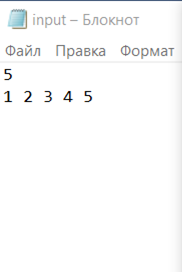
\includegraphics[scale=0.6]{input}
		\caption{Input file}
		\label{pic:pic_name} % название для ссылок внутри кода
  \end{center}
  \begin{center}
		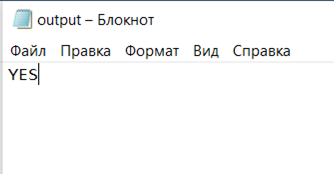
\includegraphics[scale=0.7]{output}
		\caption{Output file}
		\label{pic:pic_name} % название для ссылок внутри кода
  \end{center}
\end{figure}

\newpage
\section*{Вывод}
в лабораторной работе я встретилась с понятиями кучи и очереди с приоритетами, разобралась в их взаимосвязи и рассмотрела разные варианты реализации подобных кодов.
\addcontentsline{toc}{section}{Вывод}

% Не редактируем: Страница библиографии (формируется автоматически из книжек, указанных в refs.bib и пометок \cite{имя_источника} в тексте)
\newpage
\printbibliography[title=Список использованных источников]
\addcontentsline{toc}{section}{Список использованных источников}
\end{document}
